% !TeX spellcheck = es_MX-SpanishMexico
%----------------------------------------------------------------------------------------------------
%                           		  ENTRE LÍNEAS DE TIERRA

% Curso: Arqueología Bíblica
% Módulo 1: Introducción, Definiciones y Conceptos
% Elabora: Rodrigo Gerardo Trejo Arriaga

%----------------------------------------------------------------------------------------------------

% FORMATO DEL DOCUMENTO


\documentclass[11pt]{article} % Letra estandar

\usepackage[utf8]{inputenc}

%\usepackage{tgadventor}
%\renewcommand{\familydefault}{\sfdefault}

\usepackage[light,math]{iwona}

\usepackage[T1]{fontenc}


\usepackage[spanish]{babel}
\addto\captionsspanish{\renewcommand{\abstractname}{\large{Introducción}}}

\usepackage[margin=1in,letterpaper]{geometry}

\usepackage{fancyhdr} % Paquete para personalizar encabezado y pie de página
\pagestyle{fancy} % Establece que personalizaremos el pie de pagina y el encabezado
\setlength{\headheight}{13.59999pt} % Establece la altura del encabezado
\fancyhead[R]{\textcolor{darkBlue}{Teoría de la Computación}} % Encabezado derecho
\fancyhead[L]{\textit{\textcolor{darkBlue}{Escuela Superior de Cómputo}}} % Encabezado izquierdo
\fancyfoot[L]{\textit{\textcolor{darkBlue}{Práctica 3}}} % Pie de página izquierdo 
\fancyfoot[R]{\textcolor{darkBlue}{\thepage}} % Pie de página  derecho
\fancyfoot[C]{} % Elimina la nueración central de páginas en el pie de página
\renewcommand{\headrulewidth}{0.5pt} % Grosor de la linea de encabezado
\renewcommand{\footrulewidth}{0.5pt} % Grosor de la linea de pie de página

\usepackage{enumitem}

\usepackage{changepage}

\usepackage{graphicx}

\usepackage{tabularx}

\setlength{\parskip}{8pt}

\usepackage{xcolor}
\definecolor{darkBlue}{rgb}{0,0,0.31}
%\definecolor{darkBlue}{rgb}{0,0,0.5}
\definecolor{munsell}{rgb}{0.0, 0.5, 0.69}
\definecolor{indigo}{rgb}{0.0, 0.25, 0.42}
\renewcommand{\footrulewidth}{2pt}
\renewcommand{\footrule}{\hbox to\headwidth{\color{darkBlue}\leaders\hrule height \footrulewidth\hfill}}

\usepackage{colortbl}

\usepackage{titlesec}
\titleformat{\section}
{\normalfont\Large\bfseries\color{darkBlue}}{\thesection.}{1em}{}

\usepackage{tabularx}

\usepackage{textcomp}

\usepackage{titling}

\usepackage{apacite}
\bibliographystyle{apacite}

%\usepackage{natbib}
%\setlength{\bibsep}{6pt}

\usepackage{setspace}

\usepackage{listings}


\lstset{
	language=Python,                % Lenguaje del código (Python en este caso)
	basicstyle=\ttfamily,           % Estilo de fuente
	keywordstyle=\color{blue},      % Estilo para las palabras clave
	commentstyle=\color{green},     % Estilo para los comentarios
	numbers=left,                   % Colocar números de línea a la izquierda
	numberstyle=\tiny\color{gray},  % Estilo para los números de línea
	stepnumber=1,                   % Número de línea cada 1 línea
	tabsize=4,                      % Tamaño de la tabulación
	frame=single,                   % Colocar un marco alrededor del código
	breaklines=true,                % Romper líneas largas automáticamente
	showstringspaces=false,         % No mostrar espacios en cadenas
	escapeinside={(*@}{@*)},        % Para incluir caracteres especiales en el código
	extendedchars=true               % Permitir caracteres especiales, como acentos
}


\renewcommand{\thesection}{\Roman{section}}

%----------------------------------------------------------------------------------------------------
% CUERPO DEL DOCUMENTO

\begin{document}
	
	\begin{titlepage}
		\centering
		{
\includegraphics[width=0.25\textwidth]{descarga}\par}
		\vspace{0.5cm}
		{\bfseries\huge Escuela Superior de Cómputo \par}
		\vspace{0.7cm}
		{\scshape\LARGE Teoría de la Computación \par}
		\vspace{0.3cm}
		\vspace{3.1cm}
		{\scshape \Huge \textbf{Práctica 4:}  \par}
		\vspace{0.03cm}
		{{\LARGE \textit{Tablero}} \par}
		%\vfill
		\vspace{3.5cm}
		{\Large Autor: \par}
		{\Large Rodrigo Gerardo Trejo Arriaga \par}
		%\vfill
		\vspace{3cm}
		{\Large Octubre 2023 \par}
	\end{titlepage}
	
	\begin{center}
		\vspace*{0.1cm}
		{\huge \textcolor{darkBlue}{\textbf{Práctica 4:}} \par}
		
		{\Large \textcolor{darkBlue}{\textbf{\textit{Tablero}}}}
	\end{center}
	

Los Autómatas Finitos No Deterministas (AFND) son un concepto fundamental en la teoría de la computación y la teoría de lenguajes formales. Son una extensión de los Autómatas Finitos Deterministas (AFD) y se caracterizan por su capacidad para tener múltiples transiciones posibles desde un estado dado en respuesta a un símbolo de entrada o incluso la posibilidad de no tener una transición definida. Esto contrasta con los AFD, que siguen un proceso determinista y tienen una única transición para cada combinación de estado y símbolo.


Los componentes de un AFND son similares a los de un AFD:

\begin{itemize}
	\item \textbf{Conjunto de Estados ($Q$):} Un conjunto finito de estados que representa los diferentes estados internos de la máquina. Por ejemplo, $Q = \{q_0, q_1, q_2\}$.
	
	\item \textbf{Alfabeto de Entrada ($\Sigma$):} Un conjunto finito de símbolos utilizados como entrada. Por ejemplo, $\Sigma = \{0, 1\}$.
	
	\item \textbf{Función de Transición ($\delta$):} A diferencia de un AFD, la función de transición en un AFND puede devolver múltiples estados o incluso el estado vacío $\emptyset$. Formalmente, $\delta: Q \times \Sigma \rightarrow 2^Q$, donde $2^Q$ representa el conjunto de subconjuntos de $Q$.
	
	\item \textbf{Estado Inicial ($q_0$):} El estado en el que se encuentra la máquina al comienzo de la ejecución.
	
	\item \textbf{Conjunto de Estados Finales ($F$):} Un subconjunto de estados que se consideran estados de aceptación. Si la máquina termina en al menos uno de estos estados después de procesar la entrada, se acepta la cadena.
\end{itemize}


El proceso de reconocimiento en un AFND es similar al de un AFD, pero con la posibilidad de múltiples transiciones o la falta de transiciones en ciertos casos. Un AFND puede explorar múltiples ramas posibles durante el procesamiento de una cadena.


Una cadena se considera aceptada por un AFND si existe al menos una secuencia de transiciones que lleve a la máquina a un estado final después de procesar toda la entrada. No es necesario que todas las transiciones sean deterministas.


El lenguaje aceptado por un AFND es el conjunto de todas las cadenas que la máquina acepta, de acuerdo con la definición de aceptación anterior. Es importante destacar que un AFND puede aceptar lenguajes más generales que los AFD.


Es importante notar que cualquier lenguaje aceptado por un AFND también puede ser aceptado por un AFD. Existe un procedimiento para convertir un AFND en un AFD, lo que significa que los lenguajes regulares reconocidos por AFND y AFD son equivalentes. Sin embargo, los AFND son más expresivos y pueden representar de manera más concisa ciertos patrones en lenguajes regulares.


Al igual que los AFD, los Autómatas Finitos No Deterministas son adecuados para reconocer lenguajes regulares. No pueden reconocer lenguajes más complejos, como los lenguajes libres de contexto o los lenguajes sensibles al contexto. Para lenguajes más complejos, se utilizan otros tipos de autómatas, como los autómatas de pila o las máquinas de Turing.
	
	
	\section{Instrucciones}
	
	A continuación, se presentan las instrucciones para el programa, que debe ser capaz de ejecutarse en modo automático y manual:
	
	\begin{enumerate}
		\item \textbf{Modos de Ejecución:} El programa debe permitir dos modos de ejecución: automático y manual.
		
		\item \textbf{Entrada de Movimientos:} En el modo manual, el usuario podrá introducir la cadena de movimientos o generarla aleatoriamente.
		
		\item \textbf{Número de Piezas:} El programa puede funcionar con una pieza o dos piezas.
		
		\item \textbf{Segunda Pieza:} En el caso de dos piezas, la segunda pieza debe iniciar en el estado 4 y su estado final es el estado 13.
		
		\item \textbf{Iniciativa Aleatoria:} Cuando inicie el juego, de manera aleatoria el programa debe decidir quién inicia.
		
		\item \textbf{Generación de Archivos:} Una vez definida la cadena de movimientos para una o dos piezas, el programa debe generar dos tipos de archivos:
		
		\begin{enumerate}
			\item Archivo con todos los movimientos posibles por pieza.
			\item Archivo con todos los movimientos ganadores por pieza.
		\end{enumerate}
		
		Estos archivos servirán para reconfigurar las rutas durante el juego.
		
		\item \textbf{Reconfiguración de Rutas:} Si se reconfigura una ruta y aún así no se puede avanzar, el programa debe esperar una iteración para continuar.
		
		\item \textbf{Gráficos:} El programa debe ser capaz de graficar el tablero y mostrar los movimientos de una o dos piezas. Además, debe generar una representación gráfica de toda la red generada por los movimientos.
		
		\item \textbf{Número de Movimientos:} El número máximo de movimientos permitidos debe estar entre 4 y 50 símbolos.
	\end{enumerate}
	
	\section{Resultados}
	
	
	
	\begin{figure}[h]
		\centering
		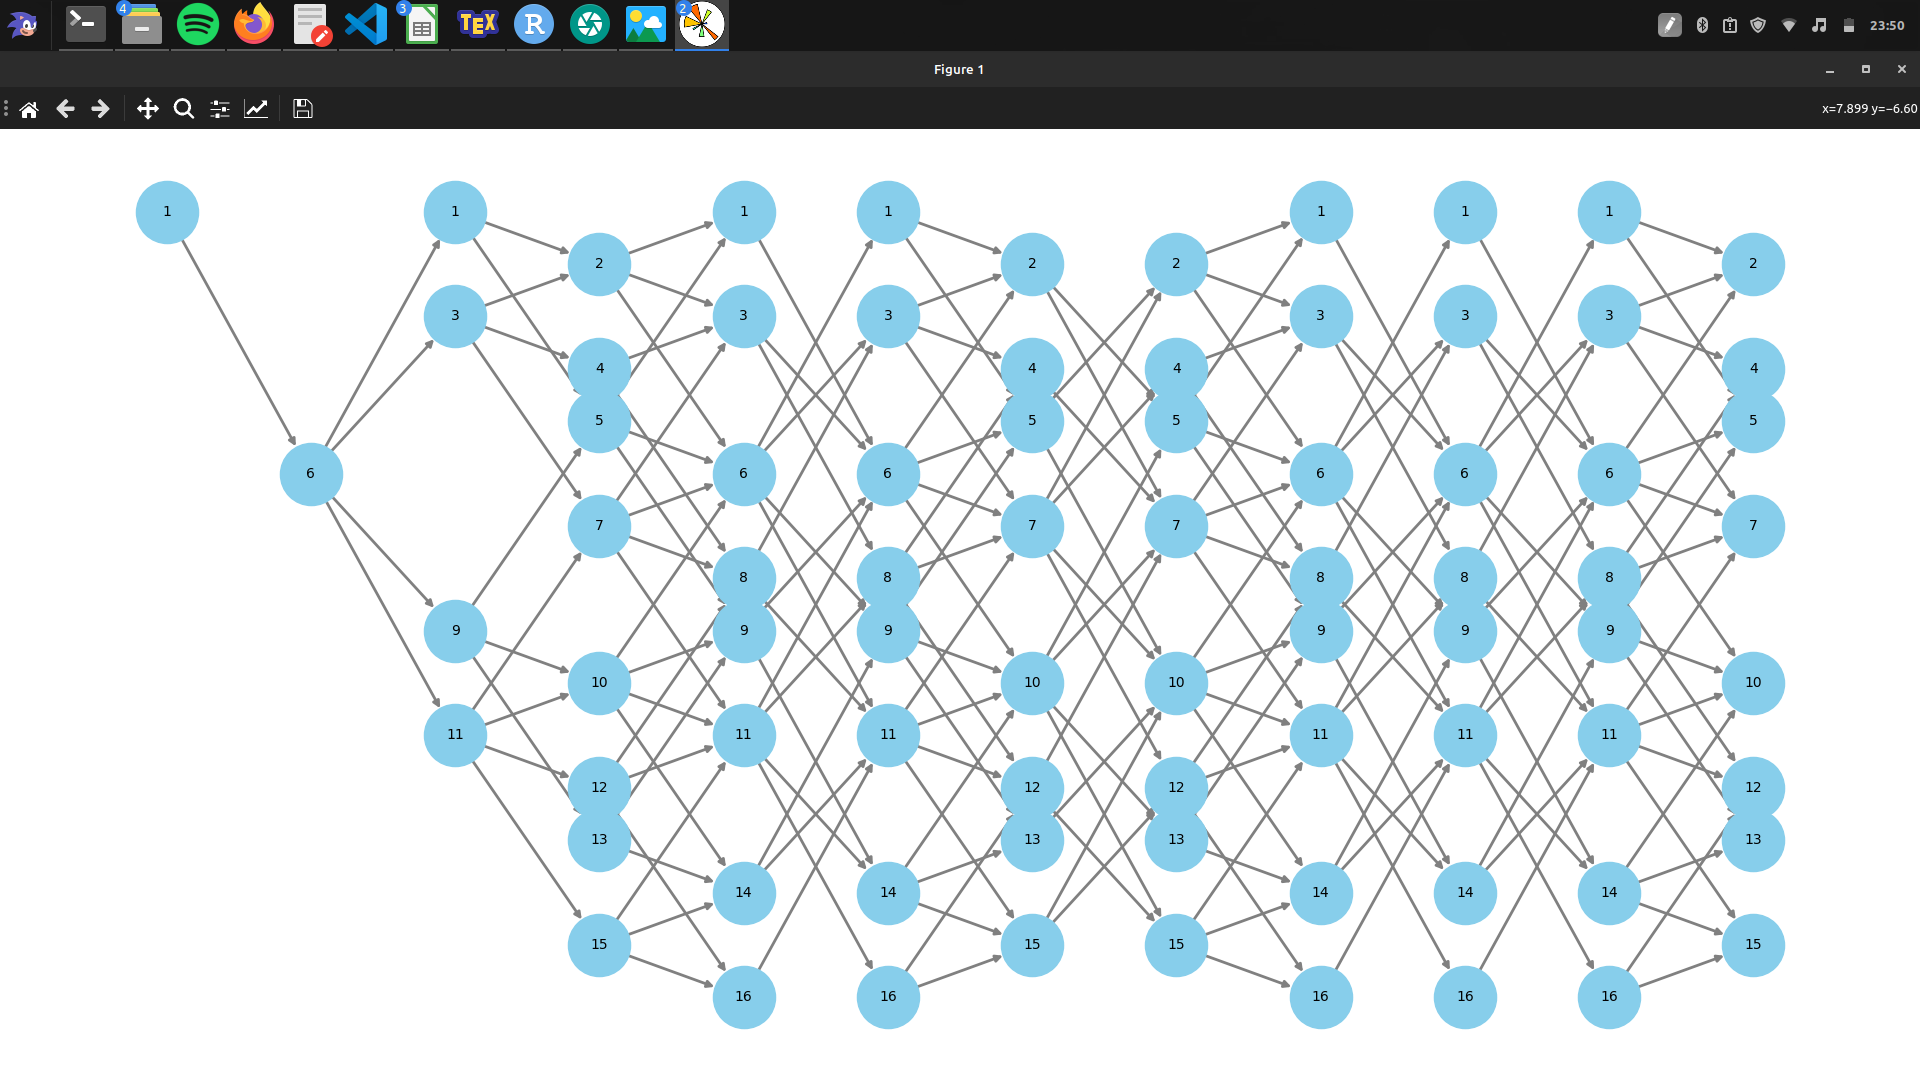
\includegraphics[width=0.8\textwidth]{imagen1.png}
		\caption{Grafo de la pieza rosa}
	\end{figure}
	
	\begin{figure}[h]
		\centering
		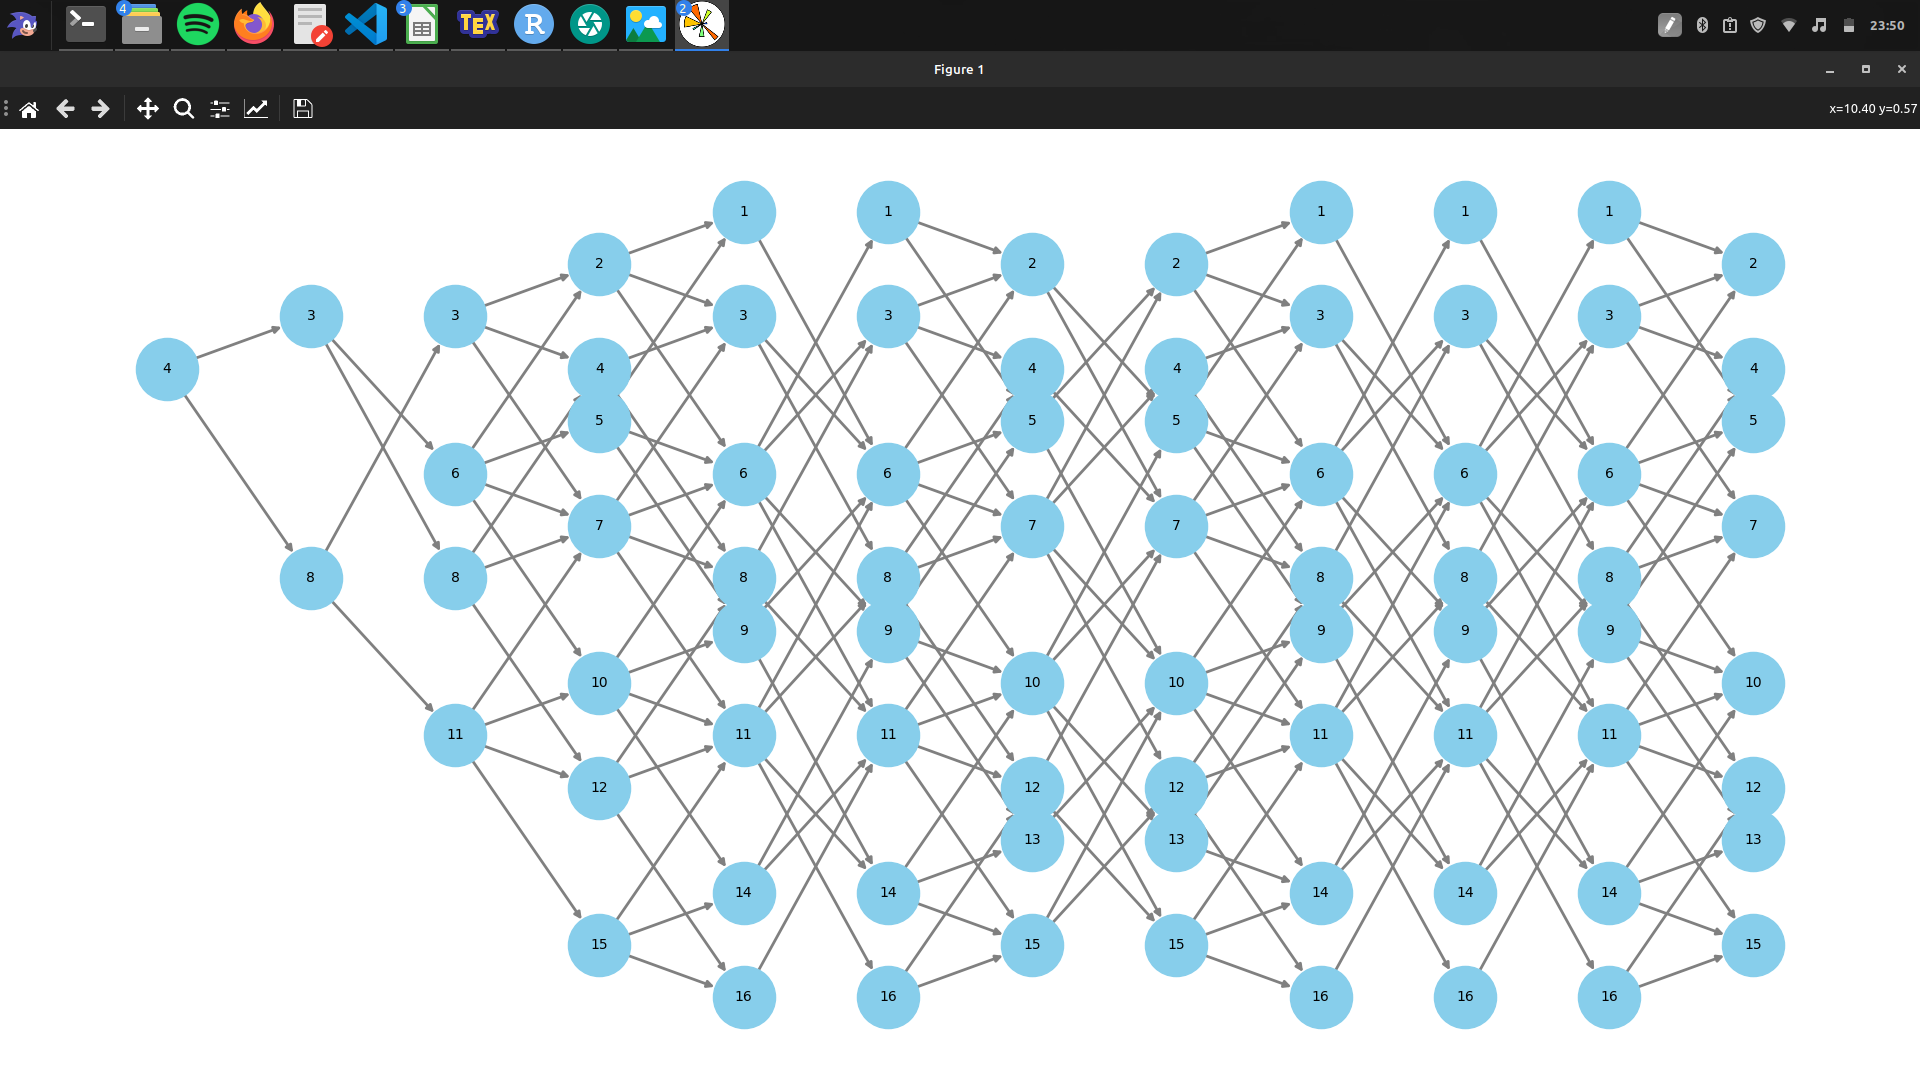
\includegraphics[width=0.8\textwidth]{imagen2.png}
		\caption{Grafo de la pieza amarilla}
	\end{figure}
	
	\begin{figure}[h]
		\centering
		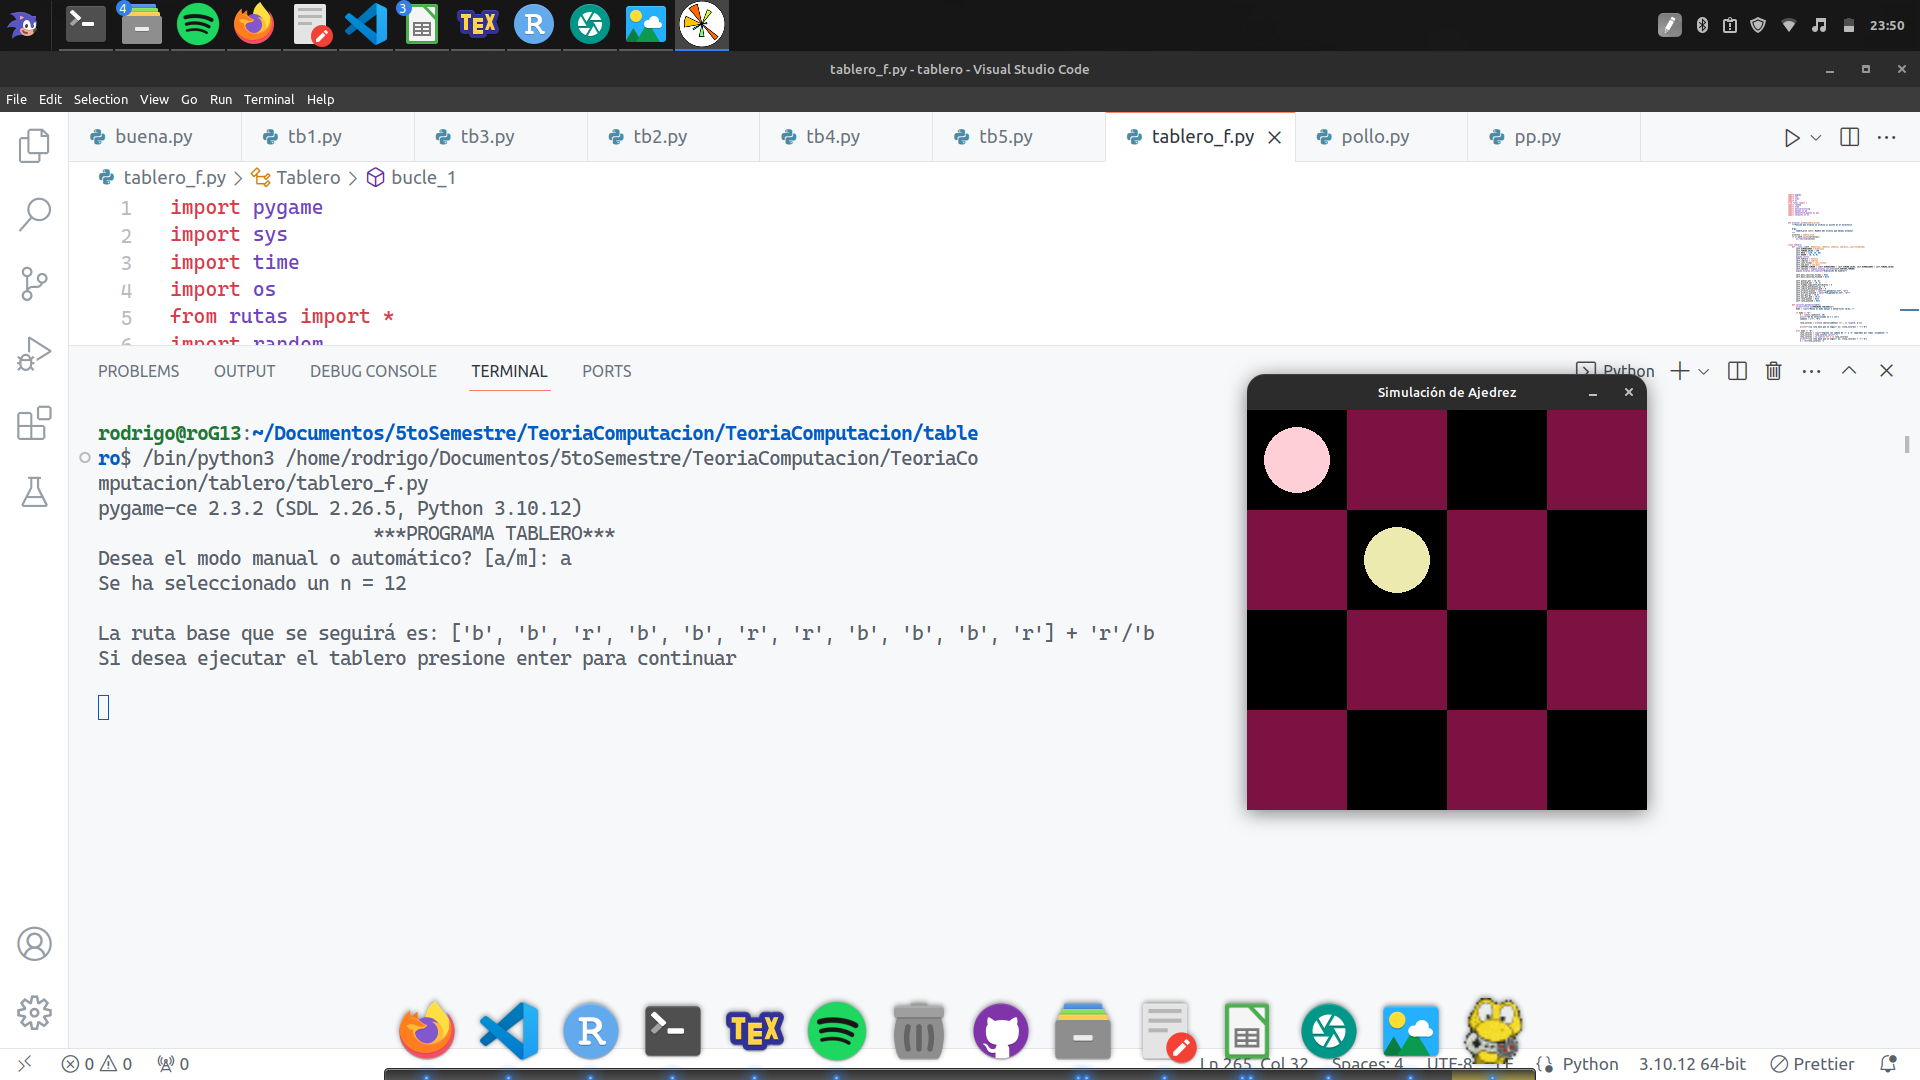
\includegraphics[width=0.8\textwidth]{imagen4.png}
		\caption{Programa en ejecución}
	\end{figure}
	
	\begin{figure}[h]
		\centering
		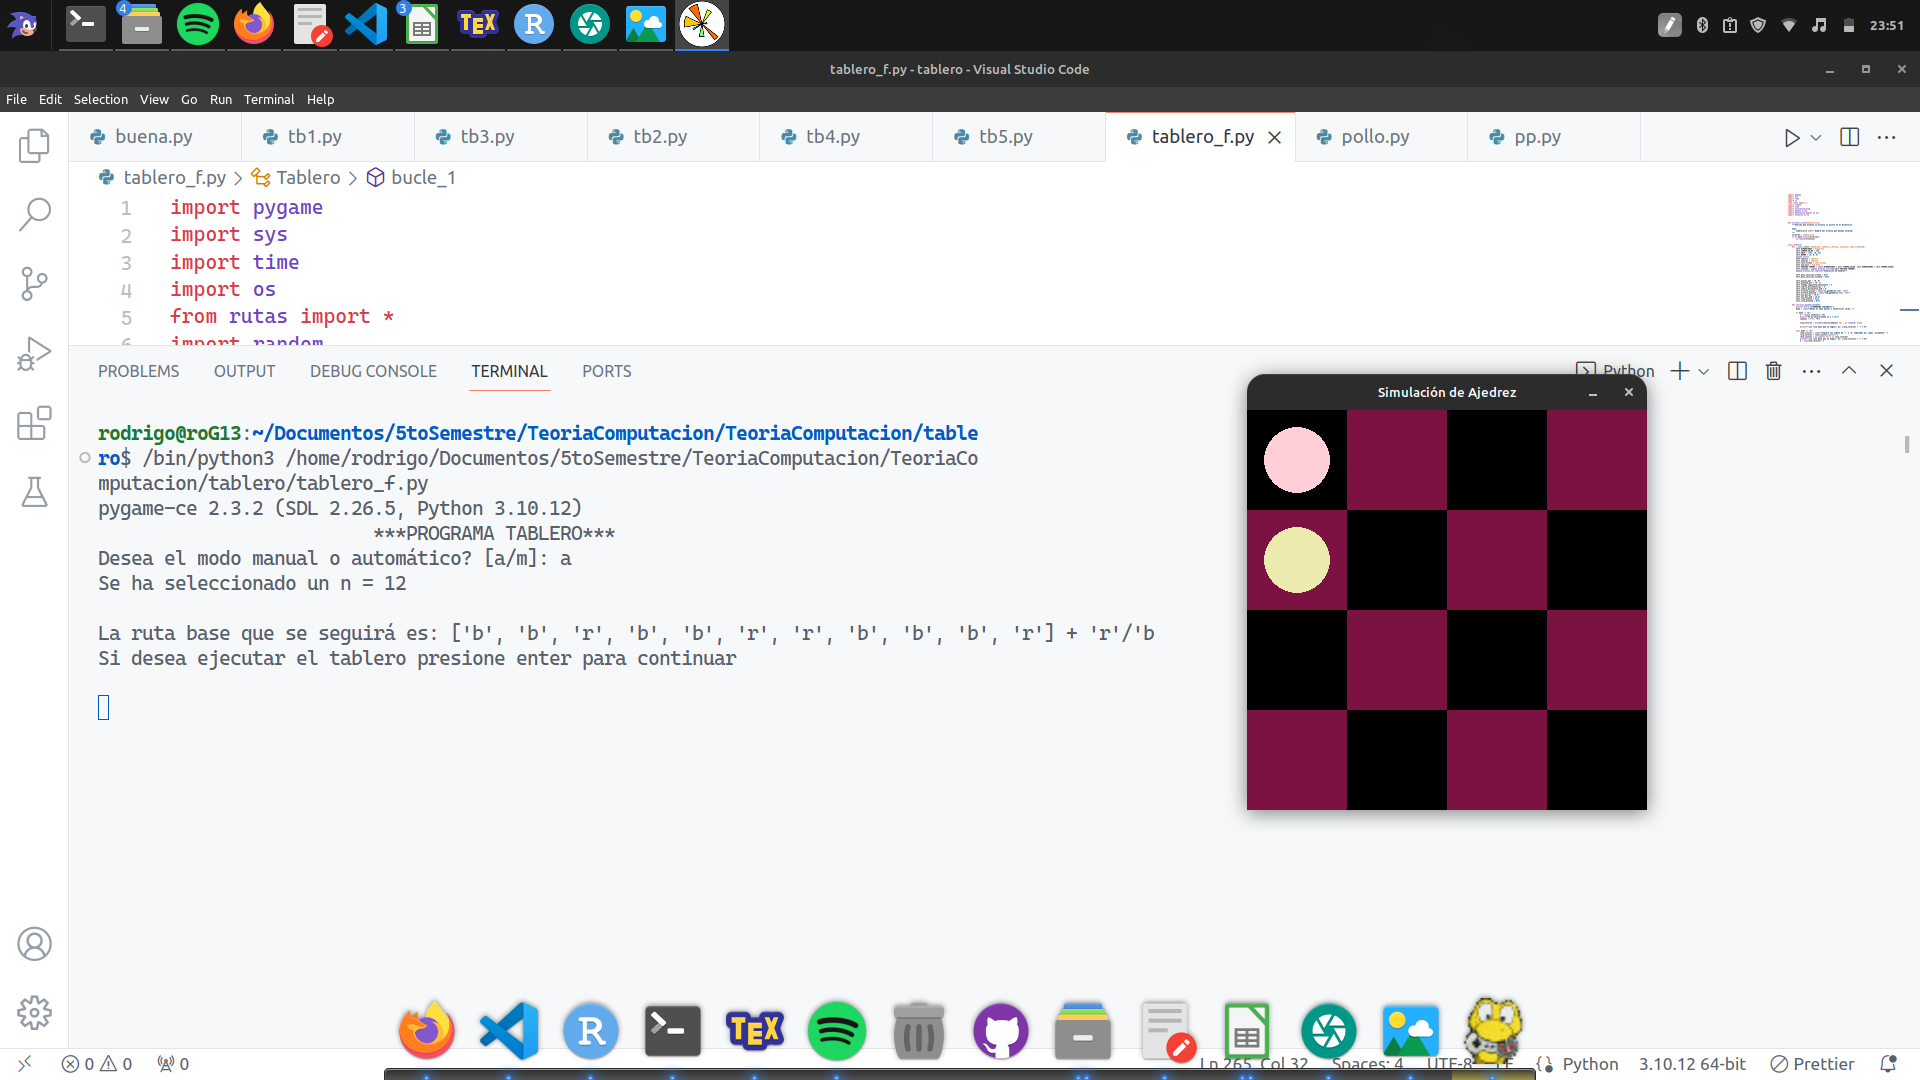
\includegraphics[width=0.8\textwidth]{imagen5.png}
		\caption{Programa en ejecución}
	\end{figure}
	
	\begin{figure}[h]
		\centering
		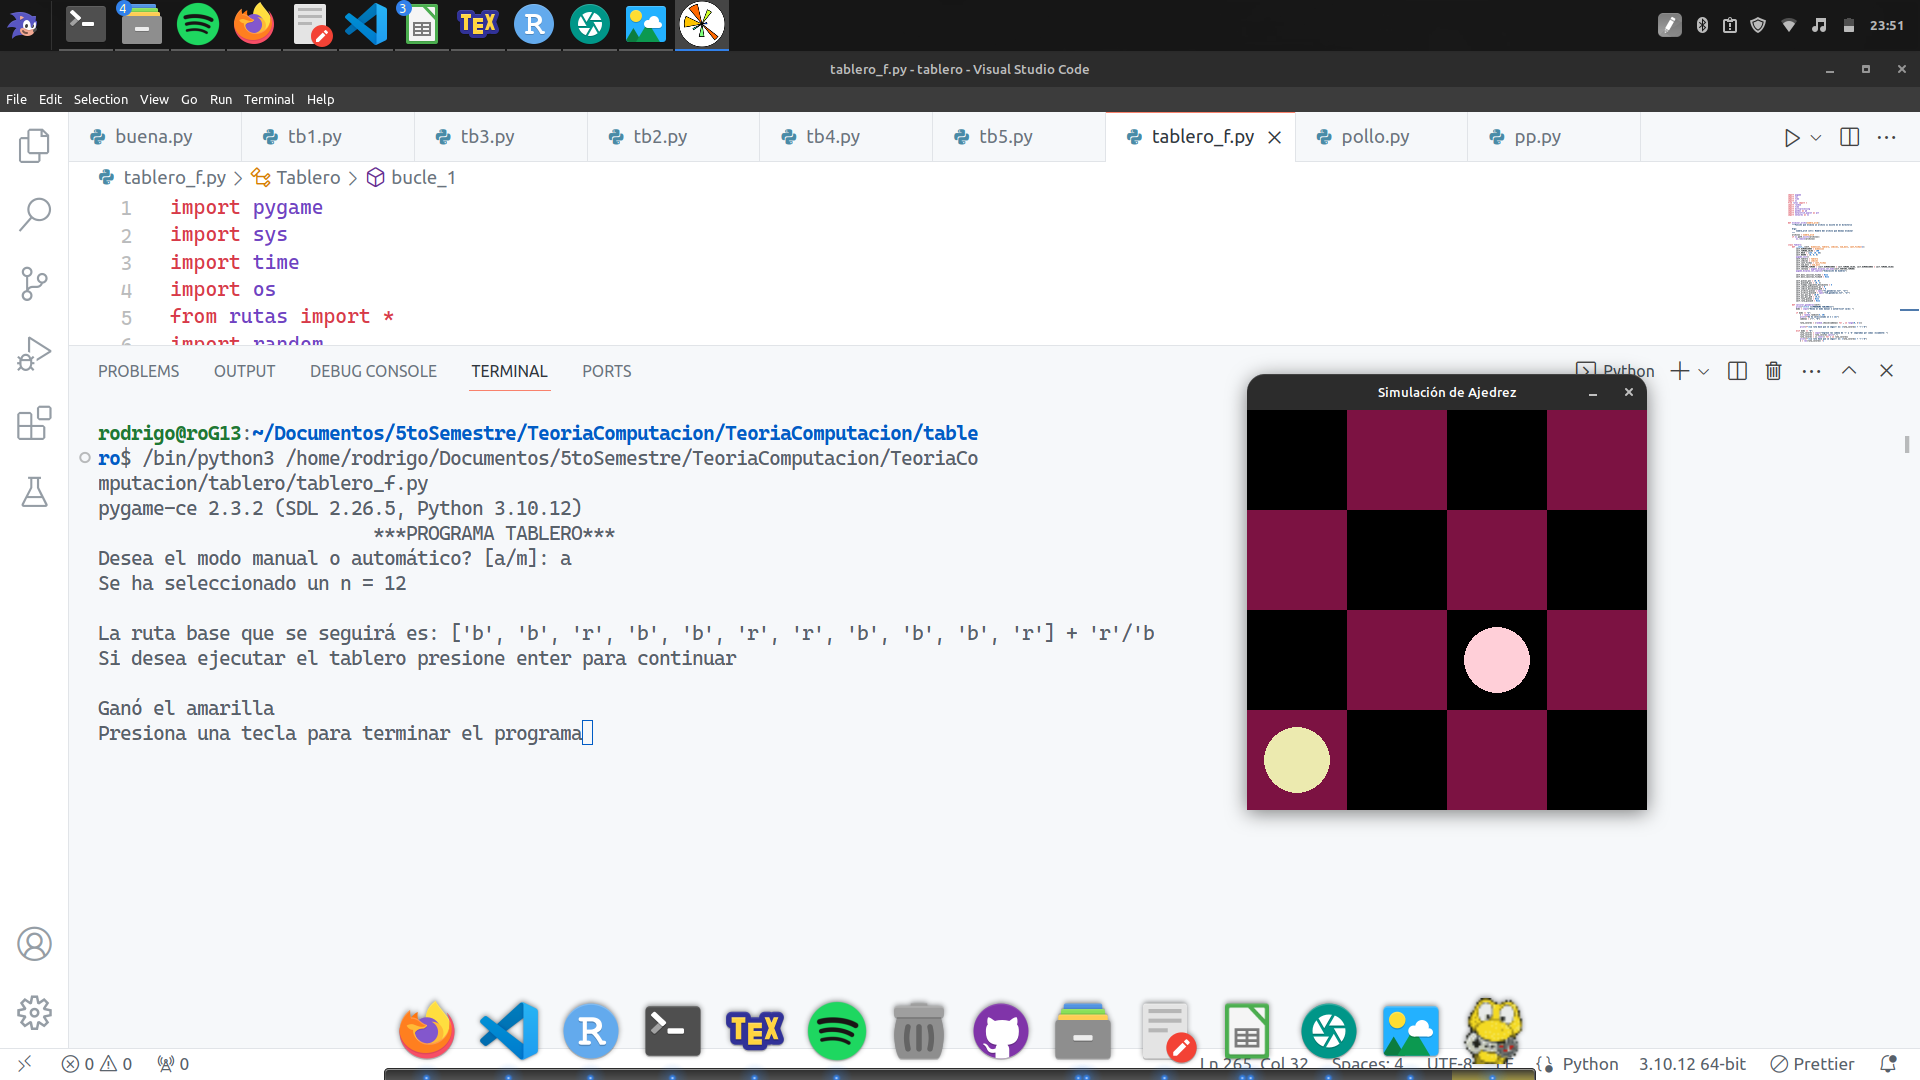
\includegraphics[width=0.8\textwidth]{imagen6.png}
		\caption{Ganó el amarillo}
	\end{figure}
	
	
	\section{Código de Implementación}
	
	\subsection{Programa principal}
	
	\begin{lstlisting}
	import pygame
	import sys
	import time
	import os
	from rutas import *
	import random
	import time
	import multiprocessing
	import pandas as pd
	import matplotlib.pyplot as plt
	import networkx as nx
	
	
	
	def eliminar_archs(nombre_arch):
	"""Función que elimina un archivo si existe en el directorio
	
	Args:
	nombre_arch (str): Nombre del archivo que deseas eliminar
	"""
	archivo1 = nombre_arch
	if os.path.exists(archivo1):
	os.remove(archivo1)
	
	
	class Tablero:
	def __init__(self, dimension, tablero, indices, num_movs, cant_fichas=1):
	self.DIMENSIONES = dimension
	self.TAMANO_CELDA = 100
	self.ROJO = (124, 18, 66)
	self.NEGRO = (0, 0, 0)
	pygame.init()
	self.tablero = tablero
	self.indices = indices
	self.cant_fichas = cant_fichas
	self.num_movs = num_movs
	self.VENTANA_TAMANO = (self.DIMENSIONES * self.TAMANO_CELDA, self.DIMENSIONES * self.TAMANO_CELDA)
	self.ventana = pygame.display.set_mode(self.VENTANA_TAMANO)
	pygame.display.set_caption("Simulación de Ajedrez")
	
	self.movs_casillas_ficha1 = None
	self.movs_casillas_ficha16 = None
	
	self.pieza1_pos = (0, 0)
	self.pieza16_pos = (0, 3)
	self.tiempo_siguiente_movimiento = 6
	self.indice_movimiento_p1 = 0
	self.indice_movimiento_p16 = 0
	self.archivo_pieza1 = open("f1_ganadoras.txt", "w+")
	self.archivo_pieza16 = open("f16_ganadoras.txt", "w+")
	self.aux_pos_p1 = (0,0)
	self.aux_pos_p16 = (0,3)
	self.ruta_pieza1 = None
	self.ruta_pieza16 = None
	
	def calcular_ganadoras(self):
	print("\t\t\t ***PROGRAMA TABLERO***")
	modo = input("Desea el modo manual o automático? [a/m]: ")
	
	if modo == "a":
	n = random.randint(4, 20)
	print(f"Se ha seleccionado un n = {n}")
	cadenas = ["r", "b"]
	
	ruta_colores = [random.choice(cadenas) for _ in range(0, n-1)]
	
	print(f"\nLa ruta base que se seguirá es: {ruta_colores} + 'r'/'b")
	
	elif modo == "m":
	ruta_colores = input("Ingrese las cadena de 'r' y 'b' separadas por comas únicamente: ")
	ruta_colores = ruta_colores.split(",")
	ruta_colores = [i.lower() for i in ruta_colores]
	print(f"\nLa ruta base que se seguirá es: {ruta_colores} + 'r'/'b")
	n = len(ruta_colores) +1
	
	
	resultados1 = {}
	resultados16 = {}
	
	q1 = multiprocessing.Queue()
	q2 = multiprocessing.Queue()
	
	generar_rutas_ficha1 = multiprocessing.Process(target=self.generar_rutas_s, args=(resultados1, tuple(self.tablero), dict(self.indices), 1, 16, ruta_colores+["b"], "f1", q1))
	generar_rutas_ficha16 = multiprocessing.Process(target=self.generar_rutas_s, args=(resultados16, tuple(self.tablero), dict(self.indices), 4, 13, ruta_colores+["r"], "f16", q2))
	
	generar_rutas_ficha1.start()
	generar_rutas_ficha16.start()
	
	self.movs_casillas_ficha1 = q1.get()
	self.movs_casillas_ficha16 = q2.get()
	generar_rutas_ficha1.join()
	generar_rutas_ficha16.join()
	self.ruta_pieza1 = self.archivo_pieza1.readline()
	self.ruta_pieza1 = self.ruta_pieza1[0: len(self.ruta_pieza1)-1].split(",")
	self.ruta_pieza16 = self.archivo_pieza16.readline()
	self.ruta_pieza16 = self.ruta_pieza16 [0: len(self.ruta_pieza16)-1].split(",")
	self.num_movs = n
	
	
	def generar_rutas_s(self, res, tablero: tuple, indices: dict, estado_inicial:int, estado_final: int, ruta_colores:list, 
	nombre_arch:str, q=None):
	
	file_lock = threading.Lock()
	variable_lock = threading.Lock()
	
	movs_casillas = {}
	
	for i in range(1, len(ruta_colores)+1):
	movs_casillas[i] = {}
	
	with open(f"{nombre_arch}_todas.txt", "w") as todas, open(f"{nombre_arch}_ganadoras.txt", "w") as ganadoras:
	resultados = threaded_generar_rutas(file_lock, variable_lock, ruta_colores, tablero, indices, estado_inicial, estado_final,todas, ganadoras, movs_casillas, res)
	for i in resultados.keys():
	todas.write("\n".join(resultados[i][0]))
	todas.write("\n")
	ganadoras.write("\n".join(resultados[i][1]))
	ganadoras.write("\n")
	
	if q:
	q.put(movs_casillas)
	return movs_casillas
	
	
	
	def dibujar_tablero(self):
	for fila in range(self.DIMENSIONES):
	for columna in range(self.DIMENSIONES):
	color = self.NEGRO if (fila + columna) % 2 == 0 else self.ROJO
	pygame.draw.rect(self.ventana, color, (columna * self.TAMANO_CELDA, fila * self.TAMANO_CELDA, self.TAMANO_CELDA, self.TAMANO_CELDA))
	
	
	def dibujar_piezas(self):
	if self.cant_fichas >= 1:
	pygame.draw.circle(self.ventana, (255, 207, 216), (self.pieza1_pos[1] * self.TAMANO_CELDA + self.TAMANO_CELDA // 2, self.pieza1_pos[0] * self.TAMANO_CELDA + self.TAMANO_CELDA // 2), self.TAMANO_CELDA // 3)
	if self.cant_fichas >= 2:
	pygame.draw.circle(self.ventana, (236, 234, 175), (self.pieza16_pos[1] * self.TAMANO_CELDA + self.TAMANO_CELDA // 2, self.pieza16_pos[0] * self.TAMANO_CELDA + self.TAMANO_CELDA // 2), self.TAMANO_CELDA // 3)
	
	
	def revisar_existencia_movs(self, num_mov, casilla_actual, evitar, casilla):
	if casilla == 1:
	for elemento in self.movs_casillas_ficha1[int(num_mov)][int(casilla_actual)]:
	if str(elemento) != str(evitar):
	return True
	else:
	for elemento in self.movs_casillas_ficha16[int(num_mov)][int(casilla_actual)]:
	if str(elemento) != str(evitar):
	return True
	return False
	
	
	def dame_mov(self, num_mov, casilla_actual, evitar, casilla):
	
	bandera_otro_mov = self.revisar_existencia_movs(num_mov, casilla_actual, evitar, casilla)
	
	if casilla == 1:
	if bandera_otro_mov:
	nueva_ruta = self.read_and_filter(f"f{casilla}_ganadoras.txt", num_mov, evitar, self.indices[self.pieza1_pos])
	return nueva_ruta
	else:
	if bandera_otro_mov:
	nueva_ruta = self.read_and_filter(f"f{casilla}_ganadoras.txt", num_mov, int(evitar), self.indices[self.pieza16_pos])
	return nueva_ruta
	
	
	
	def read_and_filter(self, file_path, n, x, y, chunk_size=10000):
	"""
	Lee un archivo en chunks y avanza hasta encontrar una fila donde en la columna "n" haya un elemento 
	distinto de x, pero en la columna "n-1" haya un elemento y. Retorna la fila encontrada 
	como un string separado por comas.
	
	Args:
	- file_path (str): Ruta al archivo.
	- n (int): Índice de la columna n.
	- x: Valor que no debe estar en la columna n.
	- y: Valor que debe estar en la columna n-1.
	- chunk_size (int): Tamaño del chunk para leer el archivo.
	
	Returns:
	- String que representa la fila encontrada o None si no se encuentra.
	"""
	
	desired_dtype = int
	
	chunk_iter = pd.read_csv(file_path, sep=',', header=None, chunksize=chunk_size)
	
	for chunk in chunk_iter:
	chunk.astype(desired_dtype)
	mask = (chunk[int(n)] != int(x)) & (chunk[int(n)-1] == int(y))
	filtered_chunk = chunk[mask]
	
	# Si encontramos al menos una fila que cumpla los criterios
	if not filtered_chunk.empty:
	# Convertir la primera fila que cumple con los criterios a string
	found_row = filtered_chunk.iloc[0]
	nueva = ','.join(map(str, found_row))
	nueva = nueva.split(",")
	return nueva
	
	# Si se recorrieron todos los chunks y no se encontró ninguna fila que cumpla los criterios
	return None
	
	
	def bucle_1(self):
	mover_pieza1 = True  # Bandera para decidir qué pieza se mueve
	tiempo_proximo_movimiento = time.time() + 2  # Inicializamos el tiempo para el primer movimiento
	
	while True:
	for evento in pygame.event.get():
	if evento.type == pygame.QUIT:
	pygame.quit()
	sys.exit()
	
	tiempo_actual = time.time()
	
	if tiempo_actual > tiempo_proximo_movimiento:
	if mover_pieza1 and self.indice_movimiento_p1 <= self.num_movs:
	aux = self.indices[int(self.ruta_pieza1[self.indice_movimiento_p1])]
	if aux != self.pieza16_pos:
	self.pieza1_pos = aux
	self.indice_movimiento_p1 += 1
	else:
	ruta = self.dame_mov(self.indice_movimiento_p1, int(self.indices[self.pieza1_pos]), int(self.indices[aux]), 1)
	if ruta is not None:
	self.ruta_pieza1 = ruta
	self.pieza1_pos = self.indices[int(self.ruta_pieza1[self.indice_movimiento_p1])]
	self.dibujar_piezas()
	self.indice_movimiento_p1 += 1
	
	if self.indice_movimiento_p1 > self.num_movs:
	print("Ganó la rosada")
	self.ventana.fill(self.ROJO)
	self.dibujar_tablero()
	self.dibujar_piezas()
	pygame.display.flip()
	input("Presione una tecla para continuar")
	input()
	break
	
	elif not mover_pieza1 and self.indice_movimiento_p16 <= self.num_movs:
	aux = self.indices[int(self.ruta_pieza16[self.indice_movimiento_p16])]
	if aux != self.pieza1_pos:
	self.pieza16_pos = aux
	self.indice_movimiento_p16 += 1
	else:
	ruta = self.dame_mov(str(self.indice_movimiento_p16), int(self.indices[self.pieza16_pos]), int(self.indices[aux]), 16)
	
	if ruta is not None:
	self.ruta_pieza16 = ruta
	aux = self.indices[int(self.ruta_pieza16[self.indice_movimiento_p16])]
	self.pieza16_pos = self.indices[int(self.ruta_pieza16[self.indice_movimiento_p16])]
	self.ventana.fill(self.ROJO)
	self.dibujar_tablero()
	self.dibujar_piezas()
	pygame.display.flip()
	self.indice_movimiento_p16 += 1
	
	if self.indice_movimiento_p16 > self.num_movs:
	print("Ganó el amarilla")
	self.ventana.fill(self.ROJO)
	self.dibujar_tablero()
	self.dibujar_piezas()
	pygame.display.flip()
	input("Presiona una tecla para terminar el programa")
	input()
	break
	
	# Cambiamos la bandera para el próximo movimiento y ajustamos el tiempo
	mover_pieza1 = not mover_pieza1
	tiempo_proximo_movimiento = tiempo_actual + 2
	
	
	
	self.ventana.fill(self.ROJO)
	self.dibujar_tablero()
	self.dibujar_piezas()
	pygame.display.flip()
	
	
	def dibujar_red_neuronal(self, data):
	G = nx.DiGraph()
	pos = {}
	layers = list(data.keys())
	
	for i, layer in enumerate(layers):
	states = list(data[layer].keys())
	for state in states:
	G.add_node(f"{layer}-{state}", label=str(state))
	pos[f"{layer}-{state}"] = (i, -state)  # (x,y) coordenadas
	
	next_layer = layer + 1
	if next_layer in data:  # Verificar si existe la siguiente capa
	for connection in data[layer][state]:
	if connection in data[next_layer]:  # Verificar si el estado de conexión existe en la siguiente capa
	G.add_edge(f"{layer}-{state}", f"{next_layer}-{connection}")
	
	labels = {node: G.nodes[node]['label'] for node in G.nodes()}
	
	# Dibuja el grafo
	plt.figure(figsize=(10, 6))
	nx.draw(G, pos, labels=labels, node_size=2000, node_color="skyblue", font_size=10, width=2, edge_color="gray")
	plt.title("Grafo tipo Red Neuronal")
	plt.show()
	
	
	
	if __name__ == "__main__":
	
	eliminar_archs("f1_ganadoras.txt")
	eliminar_archs("f1_todas.txt")
	eliminar_archs("f16_ganadoras.txt")
	eliminar_archs("f16_todas.txt")
	
	tablero = (
	(("b", False, 1), ("r", False, 2), ("b", False, 3), ("r", False, 4)),
	(("r", False, 5), ("b", False, 6), ("r", False, 7), ("b", False, 8)),
	(("b", False, 9), ("r", False, 10), ("b", False, 11), ("r", False, 12)),
	(("r", False, 13), ("b", False, 14), ("r", False, 15), ("b", False, 16))
	)
	
	indices = {1: (0,0), 2: (0,1), 3: (0,2), 4: (0,3),
		5: (1,0), 6: (1,1), 7: (1,2), 8: (1,3),
		9: (2,0), 10: (2,1), 11: (2,2), 12: (2,3),
		13: (3,0), 14: (3,1), 15: (3,2), 16: (3,3),
		(0,0):1, (0,1):2, (0,2):3, (0,3):4,
		(1,0):5, (1,1):6, (1,2):7, (1,3):8,
		(2,0):9,(2,1):10,(2,2):11,(2,3):12,
		(3,0):13, (3,1):14,(3,2):15,(3,3):16}
	
	
	juego = Tablero(4, tablero, indices, 0, cant_fichas=2)
	juego.calcular_ganadoras()
	juego.dibujar_red_neuronal(juego.movs_casillas_ficha1)
	juego.dibujar_red_neuronal(juego.movs_casillas_ficha16)
	print("Si desea ejecutar el tablero presione enter para continuar")
	juego.bucle_1()
	
	

		
		
	\end{lstlisting}
	
	\subsection{Generador de rutas}
	\begin{lstlisting}
	import threading
	
	def crear_matriz_ventanita(tablero, fila, col):
	ventanita = []
	for i in range(fila - 1, fila + 2):
	fila_aux = []
	for j in range(col - 1, col + 2):
	if 0 <= i < len(tablero) and 0 <= j < len(tablero[0]):
	fila_aux.append(tablero[i][j])
	else:
	fila_aux.append([None, None, None])
	ventanita.append(fila_aux)
	ventanita[1][1] = [None, None, None]
	return ventanita
	
	def seleccionar_hijos(estado, tablero, indices, movimientos, contador):
	fila, col = indices[estado]
	ventanita = crear_matriz_ventanita(tablero, fila, col)
	hijos = []
	for fila in ventanita:
	for casilla in fila:
	if casilla[0] == movimientos[contador]:
	hijos.append(casilla[2])
	return hijos
	
	def generar_rutas(file_lock, variable_lock,movs_casillas, movimientos, tablero, indices, estado, ruta, estado_final, todas, ganadoras, lista_estados, lista_ganadoras):
	cte = 1000000
	
	if len(ruta) <= len(movimientos):
	hijos = seleccionar_hijos(estado, tablero, indices, movimientos, len(ruta)-1)
	
	for hijo in hijos:
	with variable_lock:
	crear_bifu(movs_casillas, len(ruta), ruta[-1])
	movs_casillas[len(ruta)][ruta[-1]].add(int(hijo))
	generar_rutas(file_lock, variable_lock,movs_casillas, movimientos, tablero, indices, hijo, ruta + [hijo], estado_final, todas, ganadoras, lista_estados, lista_ganadoras)
	
	else:
	if len(lista_estados) < cte:
	lista_estados.append(f"{','.join(map(str, ruta))}")
	elif len(lista_estados) >= cte:
	lista_estados.append(f"{','.join(map(str, ruta))}")
	with file_lock:
	todas.write("\n".join(lista_estados))
	todas.write("\n")
	lista_estados.clear()
	
	if str(ruta[-1]) == str(estado_final) and len(lista_ganadoras) < cte:
	lista_ganadoras.append(f"{','.join(map(str, ruta))}")
	elif ruta[-1] == estado_final and len(lista_ganadoras) >= cte:
	lista_ganadoras.append(f"{','.join(map(str, ruta))}")
	with file_lock:
	ganadoras.write("\n".join(lista_ganadoras))
	ganadoras.write("\n")
	lista_ganadoras.clear()
	
	def crear_bifu(dict_movs, num_mov, llave):
	if llave not in dict_movs[num_mov]:
	dict_movs[num_mov][llave] = set()
	
	def threaded_generar_rutas(file_lock, variable_lock, movimientos, tablero, indices, estado_inicial, estado_final, todas, ganadoras, movs_casillas, resultados={}):
	
	ruta = [estado_inicial]
	hilos = {}
	
	hijos_iniciales = seleccionar_hijos(estado_inicial, tablero, indices, movimientos, 0)
	
	if hijos_iniciales == 1:
	ruta = [estado_inicial, hijos_iniciales[0]]
	crear_bifu(movs_casillas, len(ruta), ruta[-1])
	movs_casillas[len(ruta)][ruta[-1]].add(hijos_iniciales[0])
	hijos_iniciales = seleccionar_hijos(estado_inicial, tablero, indices, movimientos, 1)
	
	for hijo in hijos_iniciales:
	resultados[hijo] = [list(), list()]
	with variable_lock:
	crear_bifu(movs_casillas, len(ruta), ruta[-1])
	movs_casillas[len(ruta)][ruta[-1]].add(int(hijo))
	hilo = threading.Thread(target=generar_rutas, args=(file_lock, variable_lock,movs_casillas, movimientos, tablero, indices, hijo, ruta+[hijo], estado_final, todas, ganadoras, resultados[hijo][0], resultados[hijo][1]))
	hilos[hijo] = hilo
	hilo.start()
	
	for _, hilo in hilos.items():
	hilo.join()
	
	return resultados
	
	if __name__ == "__main__":
	tablero = (
	(("b", False, 1), ("r", False, 2), ("b", False, 3), ("r", False, 4)),
	(("r", False, 5), ("b", False, 6), ("r", False, 7), ("b", False, 8)),
	(("b", False, 9), ("r", False, 10), ("b", False, 11), ("r", False, 12)),
	(("r", False, 13), ("b", False, 14), ("r", False, 15), ("b", False, 16))
	)
	
	indices = {1: (0,0), 2: (0,1), 3: (0,2), 4: (0,3),
		5: (1,0), 6: (1,1), 7: (1,2), 8: (1,3),
		9: (2,0), 10: (2,1), 11: (2,2), 12: (2,3),
		13: (3,0), 14: (3,1), 15: (3,2), 16: (3,3)}
	
	with open("todas.txt", "w") as todas, open("ganadoras.txt", "w") as ganadoras:
	file_lock = threading.Lock()
	variable_lock = threading.Lock()
	ruta_colores = ['r', 'b', 'b', 'r', 'b', 'b', 'r', 'b', 'b', "r"]
	
	movs_casillas = {}
	
	for i in range(1, len(ruta_colores)+1):
	movs_casillas[i] = {}
	
	resultados = threaded_generar_rutas(file_lock, variable_lock, ruta_colores, tablero, indices, 1, 9, todas, ganadoras, movs_casillas)
	
	for i in resultados.keys():
	todas.write("\n".join(resultados[i][0]))
	todas.write("\n")
	ganadoras.write("\n".join(resultados[i][1]))
	ganadoras.write("\n")
	
	print(movs_casillas)
	print(movs_casillas)
	
	\end{lstlisting}
	
	
	
\end{document}